%!TEX root = ../thesis.tex
%*******************************************************************************
%****************************** Third Chapter **********************************
%*******************************************************************************
\graphicspath{{Chapter3/Figs/Vector/}{Chapter3/Figs/}}

%%%%%%%%%%%%%%%%%%%%%%%%%%%%%%%%%%%%%%%%%%%%%%%%%%%%%%%%%%%%%%%%%%%%%%%%%%%%%%%%
% System Architecture
%%%%%%%%%%%%%%%%%%%%%%%%%%%%%%%%%%%%%%%%%%%%%%%%%%%%%%%%%%%%%%%%%%%%%%%%%%%%%%%%
% - What is most fitting solution to integrate TPS and UI into the
%   existing architecture?
%
\chapter{System Architecture}
\section{Introduction}
The family of systems that has formed through preceding architectural design decisions forms a collection of constrained connectors ready for new systems to assimilate. Flows of information are to be aligned with adjecent system components so that dependencies are satisfied, while making use of the most fitting technologies for great adaptation. Conventions, methods and styles throughout the technical and conceptual spectrums are applied, enabling the system architecture to evolve consistently at one pace. Additionally, adjecent systems are improved by solutions introduced in this chapter.

%%%%%%%%%%%%%%%%%%%%%%%%%%%%%%%%%%%%%%%%%%%%%%%%%%%%%%%%%%%%%%%%%%%%%%%%%%%%%%%%
% Architectural Patterns
%%%%%%%%%%%%%%%%%%%%%%%%%%%%%%%%%%%%%%%%%%%%%%%%%%%%%%%%%%%%%%%%%%%%%%%%%%%%%%%%
% - Which architectural patterns fit in with the exising architecture?
%
\section{Architectural Patterns}
The current system architecture consists of three API's and nine services that connect to four databases, as can be seen in Figure \ref{fig:Architecture}. They provide functionalities to portals and mobile apps. A separation exists between user interface, business logic and data storage that is known as the three-tier or multi-tier architecture, as described in \cite{IBM-3-tier}.

\begin{figure}[H]
	\centering
	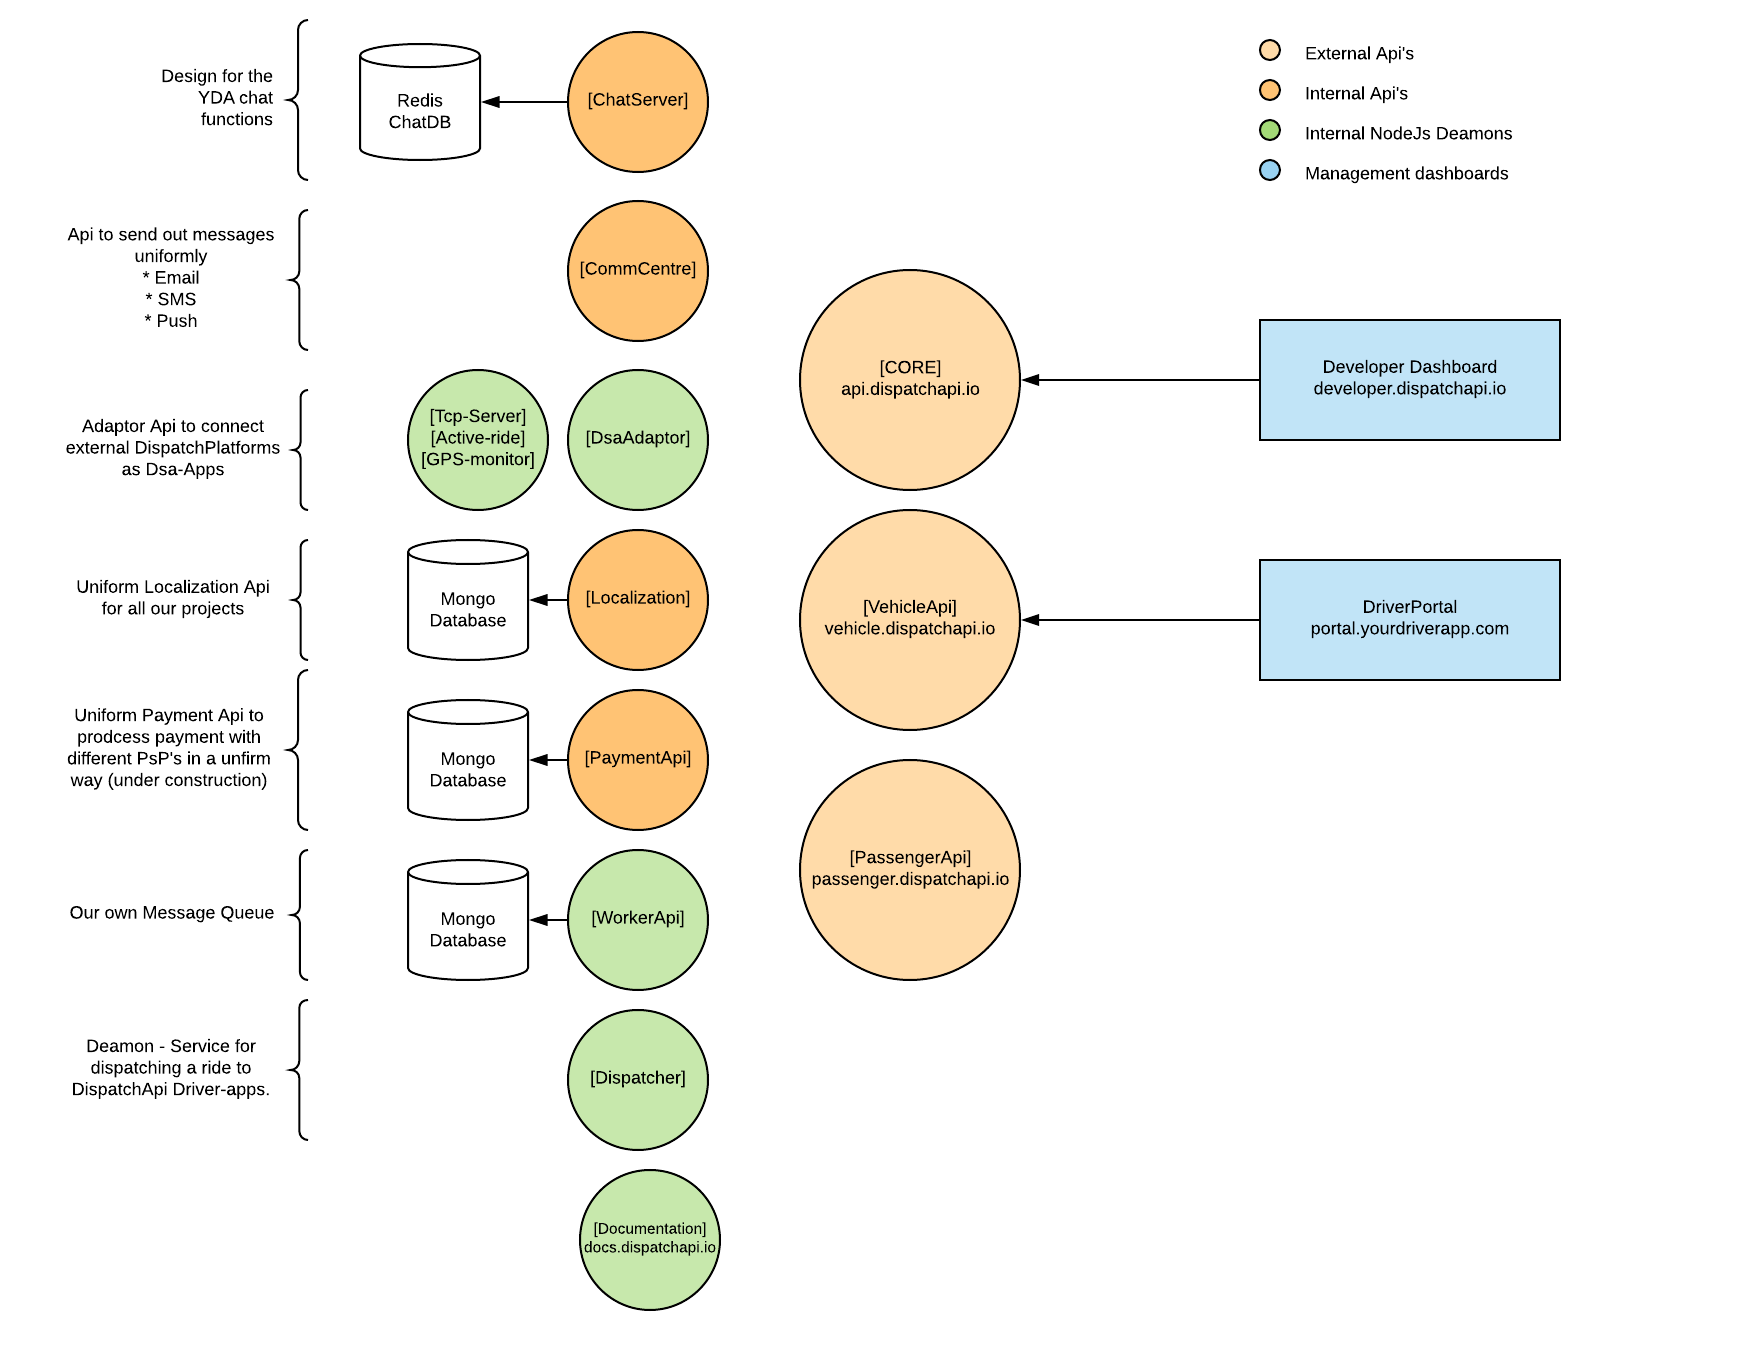
\includegraphics[width=1\textwidth]{Architecture}
	\caption[Current System Architecture]{Current System Architecture provided by taxiID.}
	\label{fig:Architecture}
\end{figure}

The bigger and smaller shapes in the Figure represent large API's and smaller services respectively. The orange colored services are used internally, the green shapes are used by external partners. The smaller services adhere to the pattern that is called service-oriented architecture, where application components provide services over a network typically.

\subsection{Monoliths}
The bigger shapes in Figure \ref{fig:Architecture} may be classified as monoliths. In the context of computer software, a monolithic system may have different definitions. Rod Stephens captures the meaning of a monolithic architecture quite broadly: "In a monolithic architecture, a single program does everything. It displays the user interface, accesses data, processes customer offers, prints invoices, launches missiles, and does whatever else the application needs to do" in \cite{rod-BSE}. In general, a monolith describes a software application which is designed without modularity. Even though the frontend is separated in some cases, it fits the description most accurately. Integration of TPS could be achieved by implementing TPS as a component of a monolith. But what logically follows is either duplication, or dependencies between large systems. The first contradicts an important principle of software engineering; don't repeat yourself (DRY), the second limits scalability and independence of deployment. The legacy system has demonstrated this issue because it has its price calculation system implemented in this manner, now facing difficulties providing the price calculation functionality to newer projects.

\subsection{Microservices}
% https://resources.sei.cmu.edu/asset_files/Presentation/2016_017_001_454683.pdf
If the previous price calculation system was implemented as a service, it could have been reused or redeployed as a second separate price calculation system for YDA instead. A consensual definition of microservices does not exist, but can be defined as a development technique that structures a system architecture as multiple loosely coupled services, exactly opposing the description of a monolith. The smaller shapes in Figure \ref{fig:Architecture} can be described as miniservices or microservices. Philipp Hauer describes the advantages of independent services accurately in \cite{microservices}, mentioning; improvements in development speed through parallel development, isolated deployment and continuous delivery (CD), scalability and potential parallelism, and independence in case of failure. Fair points of criticism have been made in regard to microservices. Jan Stenberg has pointed out that microservices are information barriers in \cite{JS-microservices}, meaning that the process of implementing a new system is degraded by the sense of ownership of specific services by developers. Technical downsides that have been discussed in general are: latency, testing, deployment, security, and message formats.

\subsection{Frontend and Backend}
A model-view-controller pattern is separating the business and presentation layers in various frontend projects. The requirements state that the frontend should be integrated in multiple portals. This would mean that separate views have to be developed for each portal, or the views should be provided to the portals via iframes. In the last case, it may be beneficial to combine the frontend and backend in the same project structure. However, this would be in conflict with this three-tier pattern, which is not desired in respect to the evolution of the system architecture. Integration of the backend would mean that the core system should contain the price calculation system as a component, and separation of the backend would mean that the backend would be set up as a separate service. As an overview, the four possibilities may be listed as:

\begin{enumerate}
	\item Integrate views in existing portal, build TPS as a separate microservice
	\item Build separate service providing iframe views, build TPS as a separate microservice
	\item Integrate views in existing portal, integrate TPS as monolith component
	\item Build separate service providing iframe views, integrate TPS as monolith component
\end{enumerate}

The final decision is based on a comparison found in table 4.1.1 in Appendix \ref{appendix:pregame}. An advice is given to separate the backend, and integrate the frontend. The final conclusion of Appendix \ref{appendix:pregame} states that the decision has to be made on a higher level, as many factors outside the scope of this project play a role in the decision.

%%%%%%%%%%%%%%%%%%%%%%%%%%%%%%%%%%%%%%%%%%%%%%%%%%%%%%%%%%%%%%%%%%%%%%%%%%%%%%%%
% Information Dependencies
%%%%%%%%%%%%%%%%%%%%%%%%%%%%%%%%%%%%%%%%%%%%%%%%%%%%%%%%%%%%%%%%%%%%%%%%%%%%%%%%
%
\section{Information Dependencies}
The frontend separation or integration cases have little influence on the further design of the system. The backend separation case however, is only possible if information dependencies are satisfied. A conceptual model can be derived from the database schema design in Figure 4.7.1.1 of Appendix \ref{appendix:pregame}, see Figure \ref{fig:DataModel}. This model shows all entities and relations that make up the price calculation system.

\begin{figure}[H]
	\centering
	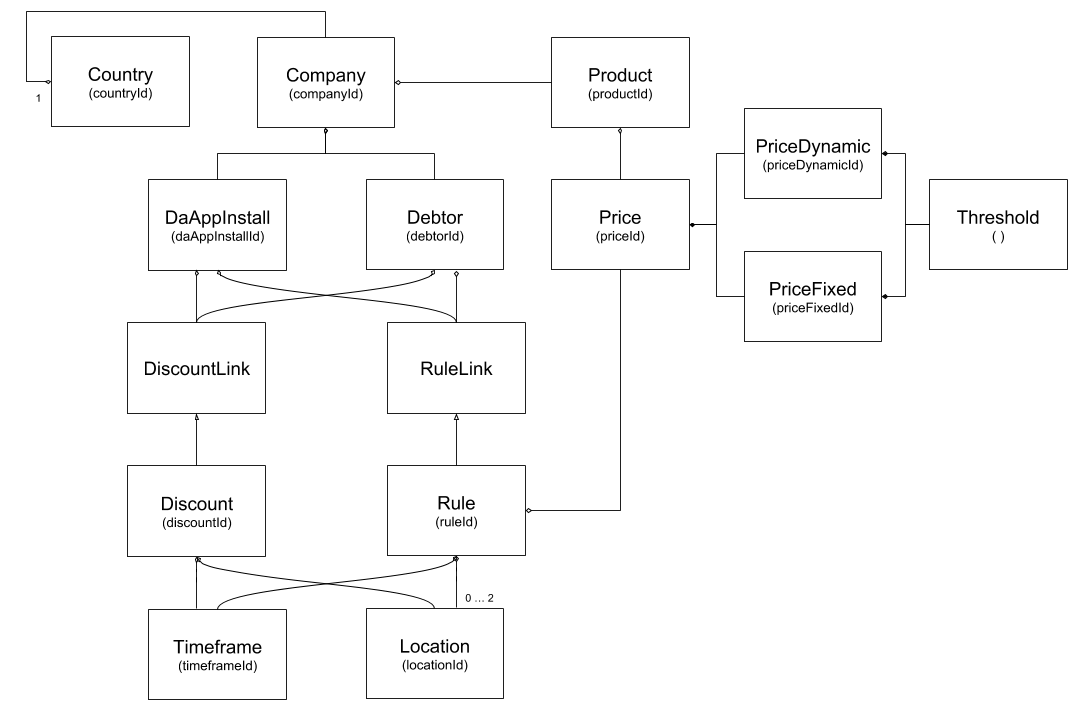
\includegraphics[width=1\textwidth]{DataModel}
	\caption[DataModel]{Conceptual data model showing database entity relations.}
	\label{fig:DataModel}
\end{figure}

In isolation, this model contains all the required information to calculate a price, provided the parameters shown in Listing \ref{lst:request}.

\begin{lstlisting}[caption={Minimal external information required for a trip price calculation.}, label={lst:request}]
	{
		"companyId": string
		"daAppInstallId": string,
		"vehicleTypes": string[],
		"passengerCount": number,
		"requestedDate": ISODate,
		"departure": { "gps": { "lat": string, "lng": string } },
		"destination": { "gps": { "lat": string, "lng": string } }
	}
\end{lstlisting}

The concrete data from the conceptual model could in theory be stored in one database, separate from the existing core database. How would the company data be synchronized? And does the system know which pricing rules should be used for the calculation? A user is identified by a combination of two identifiers: companyId and daAppInstallId. Assuming that companyId and daAppInstallId are provided in the authentication headers, the user can be identified. But this identity is futile if no pricing data is associated with it. There are three options with regard to storing the data in a way that user identity can be used to associate pricing information:

\begin{enumerate}
	\item Centralized state - a single centralized database
	\item Distributed state - multiple distributed synchronized databases
	\item Minimal state - multiple independent databases with stateless references
\end{enumerate}

A single source of truth, central database, would avoid having duplicate data all together. No synchronization, thus no network communication is neccesary, and all data is always readily available. This design desecrates the independency aspect of microservices. The multiple synchronized databases option raises the problem of having duplicate, out of sync data.

\begin{figure}[H]
	\centering
	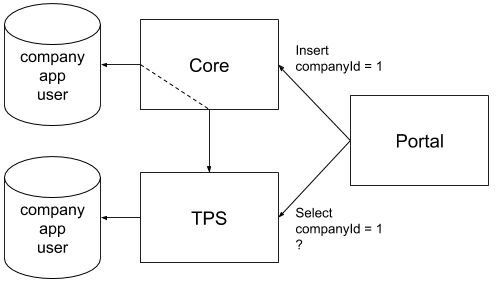
\includegraphics[width=0.6\textwidth]{DataSync}
	\caption[DataSync]{Flow of data requests.}
	\label{fig:DataSync}
\end{figure}

A one-way dataflow could reduce this problem, but it is not always entirely avoidable. This design does adhere to the concept of microservices by allowing independent deployments still. The minimal state option would improve on the previous option, by only allowing data to be referenced back in a stateless manner. This means that a company in the core database could have related data stored in the TPS database, without being 'aware' of it. The entities that reference the company can be used in an autonomous fashion, where only the neccesary information is sent to TPS whenever a request is made. Multiple proposal were made aiming to solve the combination of authentication, authorization and data consistency problems. The next section expands on the accepted solution.

%%%%%%%%%%%%%%%%%%%%%%%%%%%%%%%%%%%%%%%%%%%%%%%%%%%%%%%%%%%%%%%%%%%%%%%%%%%%%%%%
% Authentication and Authorization
%%%%%%%%%%%%%%%%%%%%%%%%%%%%%%%%%%%%%%%%%%%%%%%%%%%%%%%%%%%%%%%%%%%%%%%%%%%%%%%%
% - How can authentication between services be implemented or improved?
%
\section{Authentication and Authorization}
In the legacy system, authorization was achieved by sending extra headers for each crucial piece of information, this is clarified in Appendix \ref{appendix:pregame}, chapter 3.4. To prevent duplication, the microservice could be connected to the database that is used by the core system. But this makes the microservice less decoupled, and directly contradicts the desire to separate data dependencies. Appendix \ref{appendix:slides_2_authentication} lists four proposals, based on three proposals listed in Appendix \ref{appendix:pregame}, chapter 4.4, which are further explained in the subsections below. The third proposal is accepted, as shown in Figure \ref{fig:Authentication}. This solution closely resembles the minimal state option discussed in the previous section.

\begin{figure}[H]
	\centering
	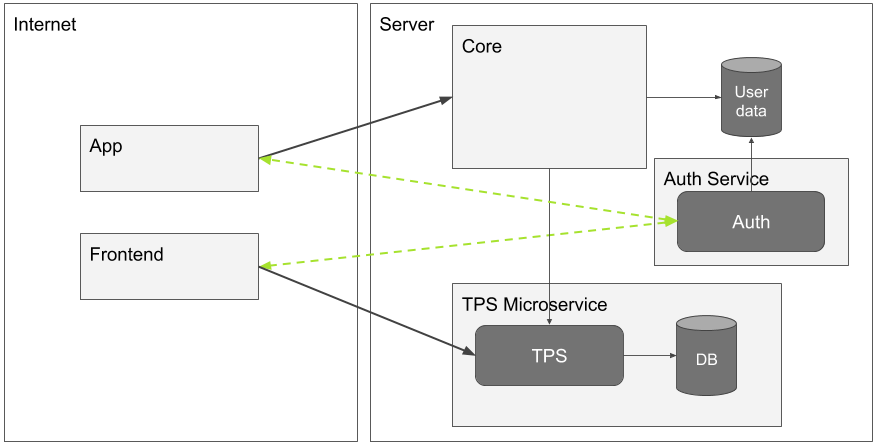
\includegraphics[width=1\textwidth]{Authentication}
	\caption[Authentication]{Accepted authentication proposal.}
	\label{fig:Authentication}
\end{figure}

The only synchronization steps are executed when a new company or application is created, or when they are deleted. The accepted proposal completely decouples the information requirements by keeping Core data and TPS data in their respective databases separated. But without the means of sharing the user identity, this solution wouldn't work. JSON Web Tokens are part of the solution that solves the problem of synchronizing user identity.

\subsection{Proposal JSON Web Token}
This proposal entirely removes the database connection to any user data. This is possible when a JSON Web Token (JWT) is used. A JWT may be signed with a cryptographic algorithm or even a public/private key pair using RSA. After the user enters valid credentials, the core system validates the credentials by comparing them with user data in the database.

\begin{lstlisting}[caption={Two user identifiers and registered claim names stored inside the payload of a JSON web token.}, label={lst:payload}]
	{
		"companyId": "59ea0846f1fea03858e16311",
		"daAppInstallId": "599d39b67c4cae5f11475e93",
		"iat": 1521729818,
		"exp": 1521816218,
		"aud": "tps.dispatchapi.io",
		"iss": "api.dispatchapi.io",
		"sub": "getPrices"
	}
\end{lstlisting}

The keys other than companyId and daAppInstallId describe expiration date of the token, and other meta information. The core system signs a token that with a secret that is known by the microservice. The token consists of three parts, separated by a fullstop. The first part (header) of the token contains information about the hashing algorithm that is used to encrypt the payload. This part is Base64Url encoded. The payload itself contains information stored in JSON format as shown in Listing \ref{lst:payload}. The identity of the user is stored in the payload that can only be revealed by whoever holds the secret with which it is signed. Then the message can be verified using the third part of the token, which is the signature. The verification step prevents tampering with the payload. Claims can be added to the payload as shown in \ref{lst:payload} to provide information about the token, as explained in \cite{JWT}.

\begin{figure}[H]
	\centering
	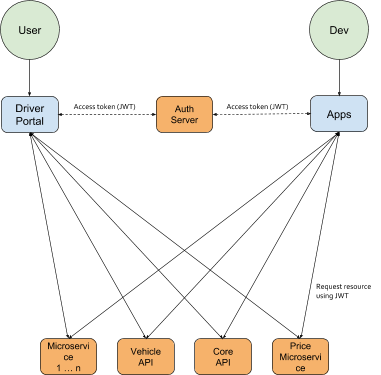
\includegraphics[width=.7\textwidth]{Auth2}
	\caption[Stateless JWT]{OAuth with stateless JWT token requests}
	\label{fig:Auth2}
\end{figure}

\subsection{Proposal OAuth 2.0}
This proposal delegates managing user identity to a separate authentication service that, similar to the pricing microservice, has its own single task of authenticating users. OAuth 2.0 is a protocol that has been designed to allow third-party apps to grant access to an HTTP service on behalf of the resource owner. This behaviour could be utilized to allow users to make use of services within the architecture, controlled by a single service, stored in a single token. A proposal is made in the Pregame document to combine oAuth with JWT and an API Gateway to introduce an automated authentication flow with a single token, instead of sending multiple headers, see Appendix \ref{appendix:pregame}.

\begin{figure}[H]
	\centering
	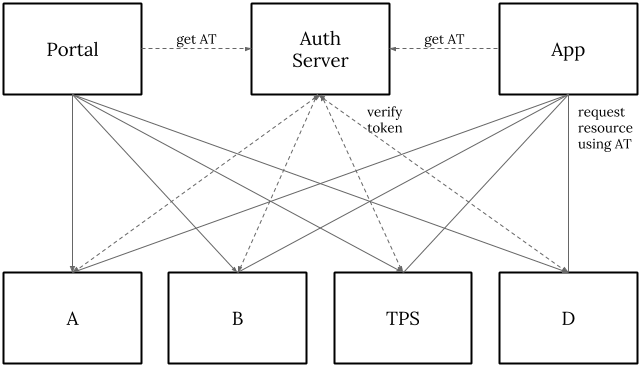
\includegraphics[width=.7\textwidth]{Auth1}
	\caption[OAuth 2.0]{OAuth requests where tokens are verified by Auth Server}
	\label{fig:Auth1}
\end{figure}

\subsection{Proposal API Gateway}
The final proposal allows services to be used by external agents is the API Gateway. It allows for a central middleware in which authentication and authorization is handled, where the microservices are shielded from public access, and all communication is established through the API Gateway \cite{api-gateway}. Next to authentication, the gateway could optimize the endpoints so that no multiple requests are needed from external agents to gather different types of resources. These calls could be made internally to the microservices behind the gateway. This also opens the possibility the freely change the microservices without changing the public endpoints exposed by the gateway, and even offers slow or instant transitions to different versions of microservices. The different proposals explain the improvements they may bring over some system. But the advice given is not tied to this project, instead to the entire Dispatch API. It’s advised to have a constructive dialogue about the future of the company, and the way it’s planning to scale. One could put a API Gateway in front of a monolithic app to help with transitioning to a microservice-oriented app.

\begin{figure}[H]
	\centering
	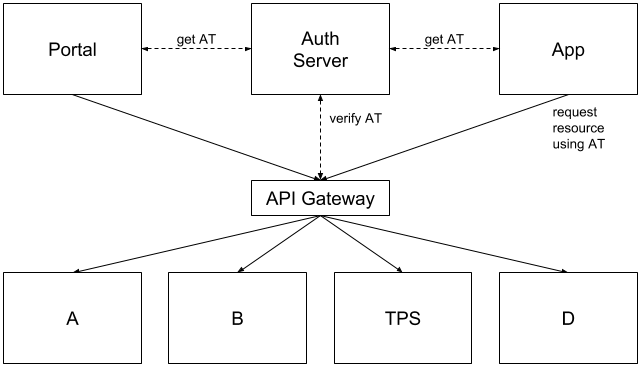
\includegraphics[width=.7\textwidth]{Auth3}
	\caption[API Gateway]{API Gateway}
	\label{fig:Auth3}
\end{figure}

This proposal is partly implemented, by sending requests via the core system.

\subsection{Reflection}

%%%%%%%%%%%%%%%%%%%%%%%%%%%%%%%%%%%%%%%%%%%%%%%%%%%%%%%%%%%%%%%%%%%%%%%%%%%%%%%%
% Languages
%%%%%%%%%%%%%%%%%%%%%%%%%%%%%%%%%%%%%%%%%%%%%%%%%%%%%%%%%%%%%%%%%%%%%%%%%%%%%%%%
%
\section{Languages}
PHP
Typescript
Java

%%%%%%%%%%%%%%%%%%%%%%%%%%%%%%%%%%%%%%%%%%%%%%%%%%%%%%%%%%%%%%%%%%%%%%%%%%%%%%%%
% Frameworks
%%%%%%%%%%%%%%%%%%%%%%%%%%%%%%%%%%%%%%%%%%%%%%%%%%%%%%%%%%%%%%%%%%%%%%%%%%%%%%%%
%
\section{Frameworks}
Loopback
NodeJS
GraphQL

An important choice that has to be made is the framework in which the project is going to be built. The team has experience with LoopBack 3.0 \cite{lb}, but considering the fact that this microservice is very small, and may not need the large amount of abstractions, Express.js is more suitable for the job. Although this means that required functionalities, that come out of the box with Loopback, have to be replaced. The API should be capable of exposing endpoints (that are going to be specified in more detail in the next phase) that are available to the DriverPortal and to external services. The endpoints for the DriverPortal should expose CRUD operations on resources that are used to calculate a trip. The endpoint for external services has only one task, given some trip information, a price has to be calculated based on the rules of the application that has been used. As mentioned, the team has experience with Loopback, and having most code written in Loopback, making it easier to transfer pieces of functionality between projects. It has a built in ORM including CRUD endpoints. On the other hand, Loopback has a steeper learning curve, stagnating velocity among external or new developers. Keeping the code base up to date may be harder because of increased amount of dependencies. There’s no clear winner. The best choice should be the result of a consensus between core developers.

The backend should be loosely coupled, but should be accessible by all users who are able to authenticate and authorize themselves. It’s advised to implement the system as a microservice, because it separates the concern effectively. By implementing the system as a module, the implementation is entirely dependent on the existing system it’s implemented in, stalling modernization of architecture in the long run. The solution that is presented in the pregame solves this challenge by having one microservice handle the requests that are in some cases routed through the DispatchAPI. The requests sent by a user from any portal should be directed at the microservice, while price calculation requests should be routed through the DispatchAPI. Loopback should be used as a framework, preferably in combination with typescript.

Angular

The first non-functional requirement states that the solution should be seamlessly integrated in the portal. On top of that, a user shouldn’t have to log in again to make use of the pricing service from within that portal. Iframes, objects and embeds have been mentioned as potential solutions to integrate a frontend in several distinct portals. This problem affects more than just the pricing project, therefore a decision must be made on a higher level before the frontend will be integrated, but the decision is not required for the first sprint to start. The options that are available are: an integrated view inside the existing DispatchAPI project or a separate solution built in Vue2 with a material design style that can be integrated using an iframe. The user interface will contain an overview showing the main concepts that a user has to maintain: pricing rules, locations, discounts. The UI should be focussed on linear navigation with overviews of detail pages. The UI will contain a screen to assign rules and discounts to DaAppInstallations and debtors, a screen to define locations, a screen to edit rules, a screen to modify vehicle types, and a screen to define timeframes.

%%%%%%%%%%%%%%%%%%%%%%%%%%%%%%%%%%%%%%%%%%%%%%%%%%%%%%%%%%%%%%%%%%%%%%%%%%%%%%%%
% Databases
%%%%%%%%%%%%%%%%%%%%%%%%%%%%%%%%%%%%%%%%%%%%%%%%%%%%%%%%%%%%%%%%%%%%%%%%%%%%%%%%
%
\section{Databases}
MySQL
MariaDB
MongoDB

MongoDB should be used over an SQL database because of its scalability. MongoDB supports geographical location types, geospatial queries including the predicate to check which polygons contain a single point, or retrieving all points contained within a single polygon.

%%%%%%%%%%%%%%%%%%%%%%%%%%%%%%%%%%%%%%%%%%%%%%%%%%%%%%%%%%%%%%%%%%%%%%%%%%%%%%%%
% Paradigms
%%%%%%%%%%%%%%%%%%%%%%%%%%%%%%%%%%%%%%%%%%%%%%%%%%%%%%%%%%%%%%%%%%%%%%%%%%%%%%%%
%
\section{Paradigms}
The object-oriented programming (OOP) paradigm offers many ways to keep a system structured. Good software design has low coupling and high cohesion, meaning that software components should have a high degree of belongingness, and a low degree of dependence in respect of eachother.

As stated in the previous chapter, another paradigm that could potentially improve the price calculation system is called: functional programming (FP).

These two paradigms together are capable of providing a modular system that is highly cohesive, and very low coupled. To understand more about the structure of the system, a class diagram visualizes the most important components in \ref{fig:ClassDiagram}.

%%%%%%%%%%%%%%%%%%%%%%%%%%%%%%%%%%%%%%%%%%%%%%%%%%%%%%%%%%%%%%%%%%%%%%%%%%%%%%%%
% Tests
%%%%%%%%%%%%%%%%%%%%%%%%%%%%%%%%%%%%%%%%%%%%%%%%%%%%%%%%%%%%%%%%%%%%%%%%%%%%%%%%
%
\section{Tests}
Mocha
Chai

%%%%%%%%%%%%%%%%%%%%%%%%%%%%%%%%%%%%%%%%%%%%%%%%%%%%%%%%%%%%%%%%%%%%%%%%%%%%%%%%
% Software Validation
%%%%%%%%%%%%%%%%%%%%%%%%%%%%%%%%%%%%%%%%%%%%%%%%%%%%%%%%%%%%%%%%%%%%%%%%%%%%%%%%
%
\section{Software Validation}

Linting is the process of running a program that will analyse code for potential errors.

Sonarqube

Buddy-Works

CircleCI

Software Reliability is defined as the probability of an item to perform a required function under stated conditions for a specified period of time. New features often introduce bugs by adding functionalities that are broken, although the reliability of the existing functionalities may also be impacted because of changes in the existing code. To prevent units of code from malfunctioning, regression tests may be implemented to validate whether a unit still functions according to a set of conditions. Static and dynamic tests may be performed using the framework Mocha \cite{mocha} and the assertion library Chai \cite{chai}. To further reduce the chances of introducing bugs, some additional techniques could be used.

%%%%%%%%%%%%%%%%%%%%%%%%%%%%%%%%%%%%%%%%%%%%%%%%%%%%%%%%%%%%%%%%%%%%%%%%%%%%%%%%
% Conclusion
%%%%%%%%%%%%%%%%%%%%%%%%%%%%%%%%%%%%%%%%%%%%%%%%%%%%%%%%%%%%%%%%%%%%%%%%%%%%%%%%
% - Which decisions could be made following the research in this chapter?
%
\section{Premise}

integration vs separation frontend
integration vs separation backend




Taking all the different aspects in this chapter into account, the advised architectural design of TPS comprises of integrated frontend views in each required portal using the associated available technologies, a separate NodeJS microservice with its own MongoDB database, Loopback as a framework to quickly implement functionalities using Typescript and a combination of OOP and FP, authentication via JWT, automated tests using mocha and chai, and continuous delivery and automated testing using Buddy-Works.

\begin{table}[htbp!]
	\centering
	\begin{tabular}{c|c|c}
		\toprule
		& MySQL & MongoDB \\
		\midrule
		Point & \checkmark & \checkmark \\
		Polygon & \checkmark & \checkmark \\
		MultiPolygon & \checkmark & \checkmark \\
		MultiPolygon & \checkmark & \checkmark \\
		MultiPolygon & \checkmark & \checkmark \\
		MultiPolygon & \checkmark & \checkmark \\
		Intersect & \checkmark & \checkmark \\
		\bottomrule
	\end{tabular}
	\caption[Databases]{Required database features.}
	\label{tab:databases}
\end{table}